\documentclass{article}
\usepackage{hyperref}
\usepackage{float}
\usepackage{graphicx}
\usepackage{tikz}
\usetikzlibrary{shapes.geometric, arrows.meta, positioning}
\tikzstyle{startstop} = [rectangle, rounded corners, minimum width=2.5cm, minimum height=1cm,text centered, draw=black, fill=blue!15]
\tikzstyle{process} = [rectangle, minimum width=2.5cm, minimum height=1cm, text centered, draw=black, fill=green!20]
\tikzstyle{decision} = [diamond, minimum width=2.5cm, minimum height=1cm, text centered, draw=black, fill=yellow!20]
\tikzstyle{arrow} = [thick,->,>=stealth]

\hypersetup{
    colorlinks=true,
    linkcolor=blue,
    urlcolor=blue,
    pdftitle=Cache Simulator,
    pdfauthor=Amber Agarwal and Anoop Singh,
    bookmarks=true,
    bookmarksopen=true
}

\date{} % No date needed

\begin{document}

% Title Page
\begin{titlepage}
    \centering
    {\LARGE \textbf{Project Report Summary}}\\[1cm]
    {\large \textbf{Assignment 3}}\\[1cm]
    \textbf{Submitted by:} \\ Amber Agarwal (2023CS50625) \\ Anoop Singh (2023CS10459)  \\[0.5cm]
    \textbf{Supervisor:} \\ Prof. Rijurekha Sen \\[1cm]
    \textbf{Institution Name} \\ IIT Delhi \\
    \textbf{Department Name} \\ Computer Science and Engineering  \\[1cm]
    
\includegraphics[height=2.5in]{th.jpg}
    \vfill
\end{titlepage}

\tableofcontents
\newpage

\section{Sections}

\subsection{Main Classes and Structures}

\begin{itemize}
    \item \textbf{Cache}: This is the core class representing a single cache instance. Each processor has its own \texttt{Cache} object that stores tag and data arrays, tracks statistics, and implements logic for handling hits, misses, invalidations, and bus transactions. Important methods include:
    \begin{itemize}
        \item \texttt{hit\_or\_miss}, \texttt{read\_hit}, \texttt{write\_hit}
        \item \texttt{read\_miss}, \texttt{write\_miss}
        \item \texttt{handle\_bus\_transaction\_completion}
    \end{itemize}

    \item \textbf{Bus}: A central shared communication medium simulating a snooping bus. It includes fields like \texttt{busy}, \texttt{cycle\_remaining}, \texttt{transaction\_type}, etc., to manage bus contention, invalidations, and cache-to-cache transfers.

    \item \textbf{Statistics}: A structure holding performance counters such as number of reads, writes, cache misses, idle cycles, data traffic, etc.

    \item \textbf{Bits}: Used to store parsed tag, index, and offset bits from an address.

    \item \textbf{Global Simulation}: The \texttt{main} function sets up four \texttt{Cache} instances (for a 4-core simulation), a shared \texttt{Bus}, and processes traces in a cycle-by-cycle fashion until all caches finish processing their instructions.
\end{itemize}

\subsection{Data Structures}

\begin{itemize}
    \item \texttt{vector<vector<CacheLineMeta>> tag\_array}: A 2D vector storing tag, state (MESI), and timestamp for each cache line.
    \item \texttt{vector<vector<vector<int>>> data\_array}: Placeholder for data blocks per set and way.
    \item \texttt{vector<pair<operation, string>> trace\_data}: Holds parsed memory accesses (read/write and address) from trace files.
\end{itemize}

\subsection{Rules Followed for the Assignment}

\begin{itemize}
    \item The MESI cache coherence protocol is used to manage consistency across caches.

    \item In case multiple cores request bus access simultaneously, the core with the lower ID is given priority.

    \item A single shared bus is assumed for the entire execution. It handles:
    \begin{itemize}
        \item Data transfer between cache and memory.
        \item Data transfer between caches (cache-to-cache).
        \item Broadcasting of coherence signals.
    \end{itemize}

    \item If the bus is busy, any core that wishes to place a request must wait until the bus becomes free.

    \item We assume:
    \begin{itemize}
        \item The sender does not stall and immediately updates its state after placing data on the bus.
        \item The receiver stalls until it receives the required data and then updates its state.
    \end{itemize}

    \item Execution cycles include:
    \begin{itemize}
        \item Time when a core actively processes its instruction.
        \item Time spent waiting for data via the bus.
    \end{itemize}

    \item Idle cycles occur when:
    \begin{itemize}
        \item A core is ready to execute an instruction but must wait for the bus.
    \end{itemize}
    
    \item No increment:
    \begin{itemize}
         \item A core has finished all its instructions (no execution or idle cycles are counted thereafter).
    \end{itemize}

    \item Cache evictions follow the LRU (Least Recently Used) policy:
    \begin{itemize}
        \item If an invalid block exists, it is replaced directly.
        \item Otherwise, the least recently used block is evicted.
        \item If the evicted block is in the \texttt{M} (Modified) state, it is first written back to memory.
        \item The eviction counter is incremented for each such replacement.
    \end{itemize}

    \item \texttt{Writeback} counter is incremented whenever a block in the \texttt{M} state is sent to memory:
    \begin{itemize}
        \item During cache eviction.
        \item When another core's read miss fetches data from this cache.
        \item When a core encounters a write miss and another core has the modified block.
    \end{itemize}

    \item \texttt{BusInvalidation} counter is incremented when:
    \begin{itemize}
        \item A core experiences a write miss or write hit.
        \item Another cache has the block in a state other than \texttt{I} (Invalid).
    \end{itemize}

    \item \texttt{BusTraffic} includes:
    \begin{itemize}
        \item All data transmitted to or from the bus.
    \end{itemize}

    \item \textbf{Bus statistics} include:
    \begin{itemize}
        \item \texttt{Total bus transactions} — count of data or signal transmissions over the bus.
        \item \texttt{Total data traffic} — sum of all bytes transferred through the bus.
    \end{itemize}
\end{itemize}




\subsection{Graphs and Analysis}

We have generated the graphs by varying four different aspects of the cache configuration to observe their impact on performance:

\begin{enumerate}
    \item \textbf{Varying the Number of Sets in the Cache:}  We increase the number of sets. This typically results in more cache hits due to improved address mapping, thereby reducing the number of execution cycles. This trend is clearly visible in the outputs for all four cores, as shown in Figure~\ref{fig:sets_variation}.
    
    \begin{figure}[H]
        \centering
        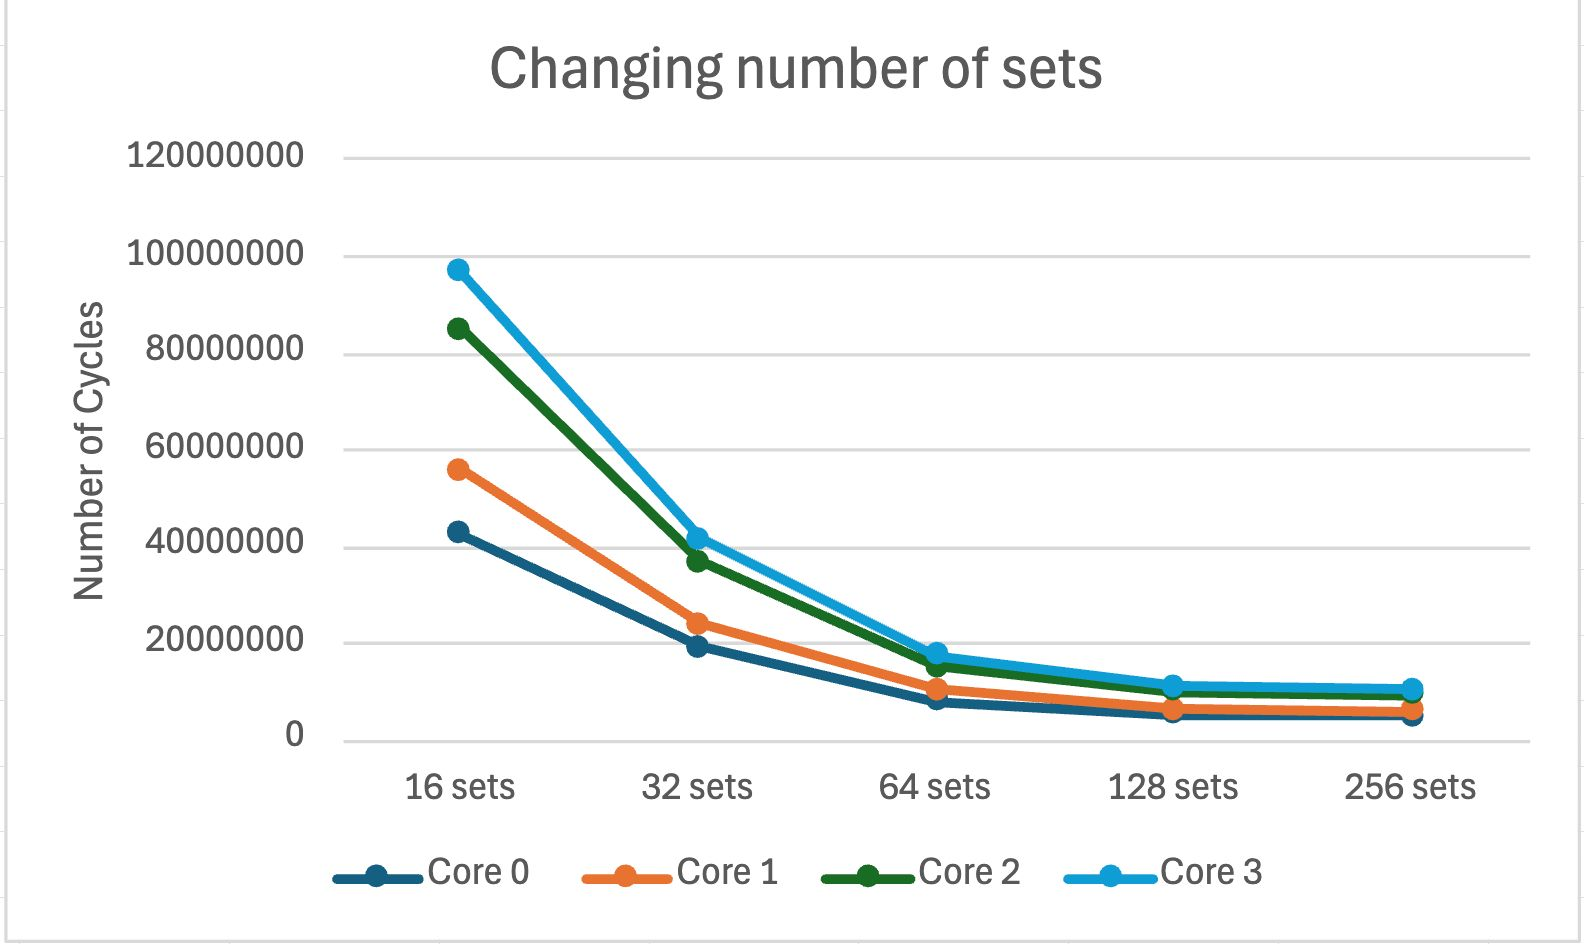
\includegraphics[width=0.7\textwidth]{1.jpeg}
        \caption{Performance variation with different numbers of cache sets}
        \label{fig:sets_variation}
    \end{figure}

    \item \textbf{Varying the Associativity of the Cache:} Increasing the associativity generally allows for better conflict resolution in set-indexed caches, which can improve cache hit rates. However, higher associativity also increases complexity and access latency. The corresponding performance implications can be seen in Figure~\ref{fig:assoc_variation}.
    
    \begin{figure}[H]
        \centering
        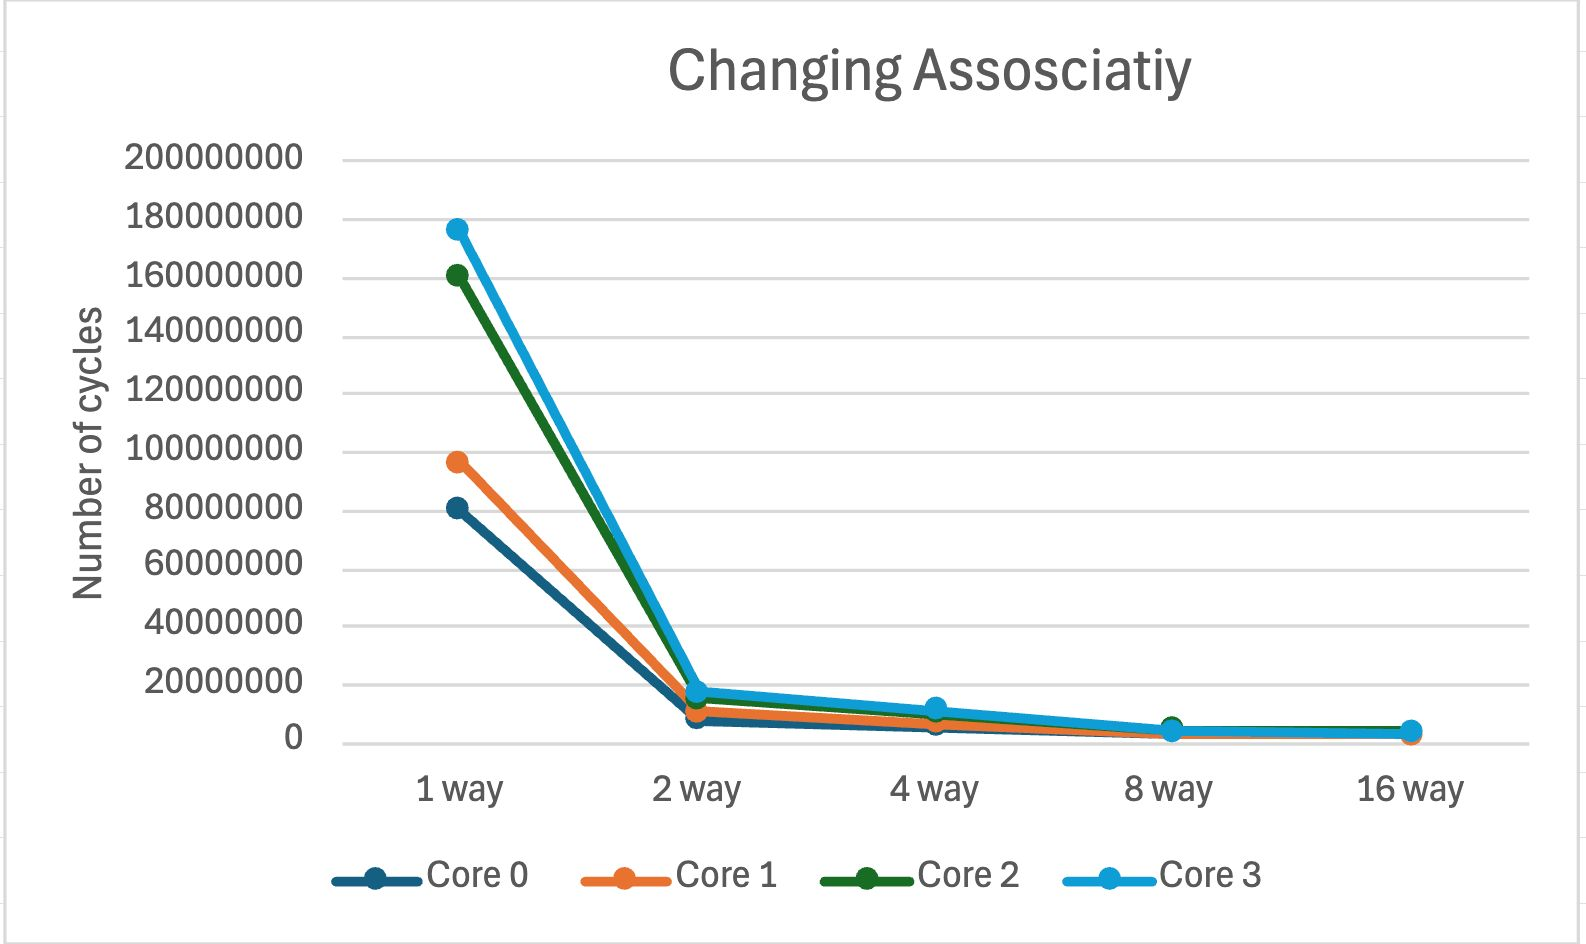
\includegraphics[width=0.7\textwidth]{2.jpeg}
        \caption{Performance variation with different cache associativity}
        \label{fig:assoc_variation}
    \end{figure}

    \item \textbf{Varying the Offset Bits in a Block:} Modifying the number of offset bits changes the block size. Larger blocks can reduce miss rates for sequential access patterns. The resulting effects on performance are illustrated in Figure~\ref{fig:offset_variation}.
    
    \begin{figure}[H]
        \centering
        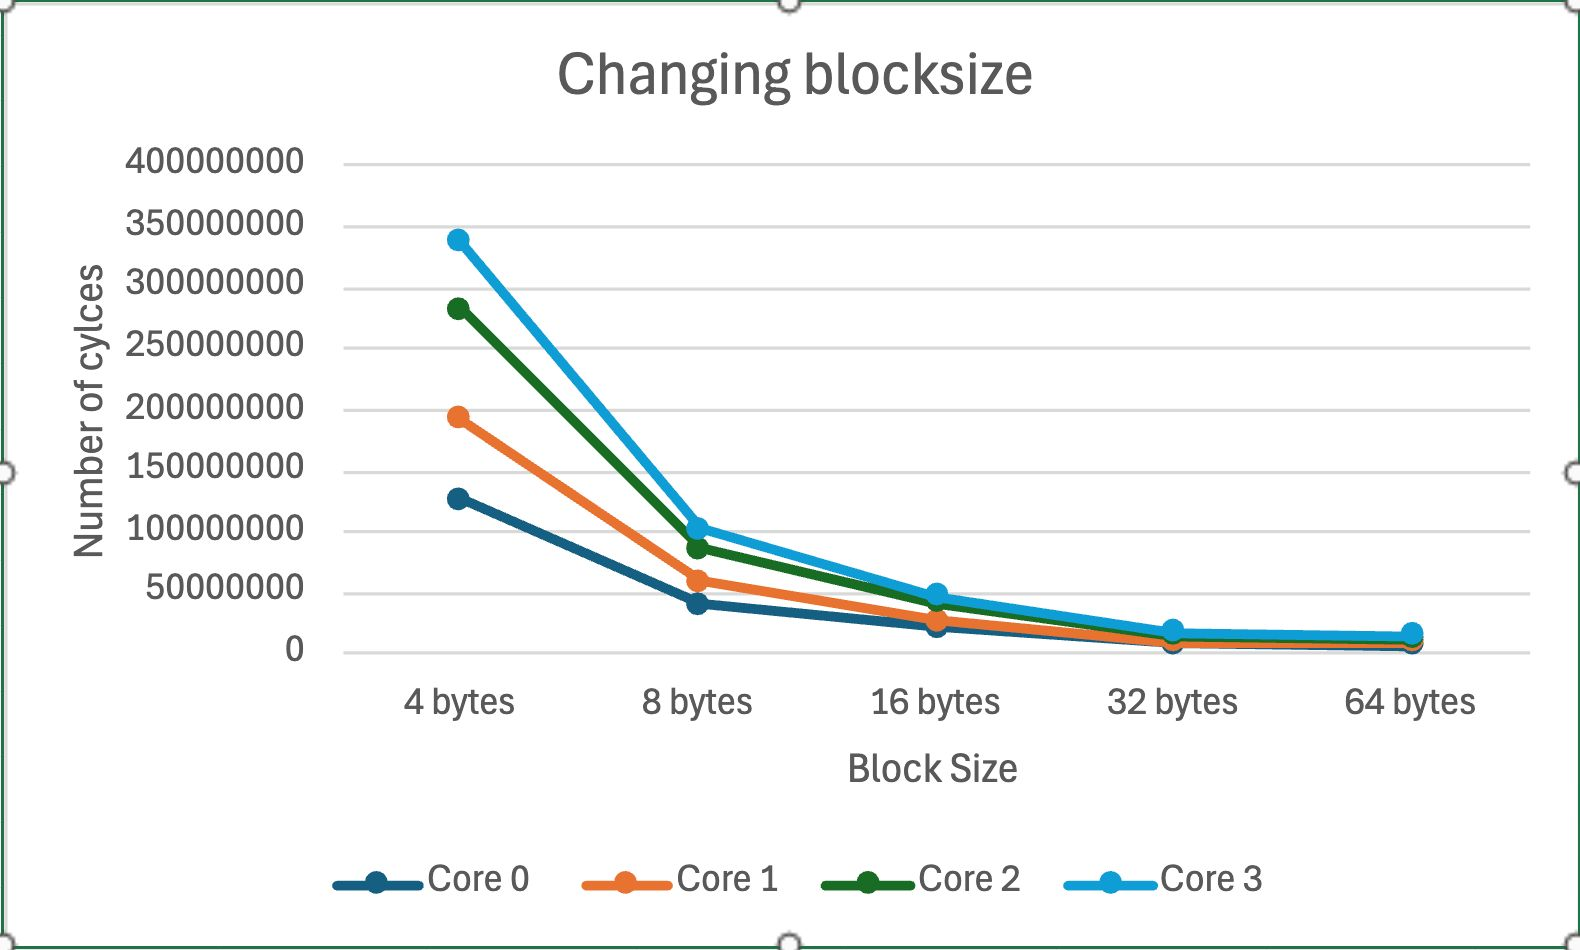
\includegraphics[width=0.7\textwidth]{3.jpeg}
        \caption{Performance variation with different block offset sizes}
        \label{fig:offset_variation}
    \end{figure}

    \item \textbf{Toggling Between Number of Sets and Associativity (with Fixed Cache Size):} In this case, we maintain the overall cache size constant and vary the configuration by adjusting the number of sets and the associativity accordingly. This trade-off allows us to analyze which combination provides optimal performance under a constrained memory budget. We see that the cycles first decrease and then increase. This behavior is due to the fact that although we reduce conflict misses, on reducing the number of sets, the blocks pointing to different sets encounter misses. The comparative results are presented in Figure~\ref{fig:fixed_size_variation}.
    
    \begin{figure}[H]
        \centering
        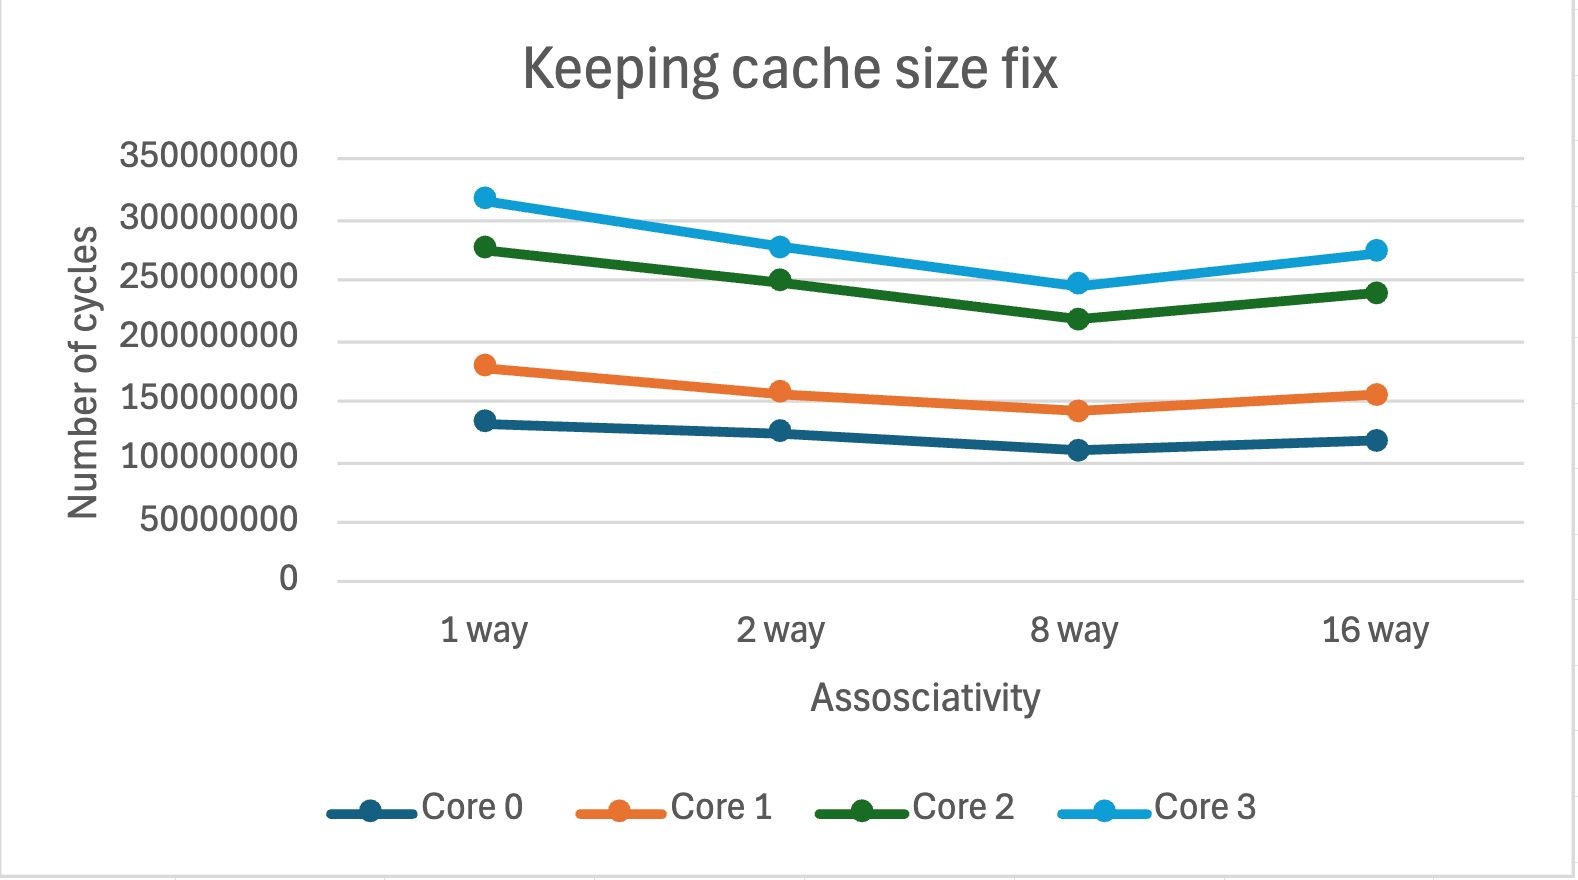
\includegraphics[width=0.7\textwidth]{4.jpeg}
        \caption{Performance variation with fixed cache size under different set/associativity configurations}
        \label{fig:fixed_size_variation}
    \end{figure}
\end{enumerate}
\subsection{Observations}

\begin{itemize}
    \item Across all the performance graphs, we observe that \textbf{Core 3 consistently incurs the highest number of execution cycles}, resulting in the longest completion time among all cores.
    
    \item This outcome is primarily due to the bus arbitration policy adopted in our simulator, which \textbf{prioritizes cores based on ascending core ID} in the event of simultaneous bus access requests.
    
    \item As a result, Core 0 always receives the highest priority, followed by Cores 1, 2, and finally 3. This fixed ordering causes Core 3 to frequently wait the longest for bus access, leading to increased idle time and total execution cycles.
    
    \item The assignment also required us to run the simulator 10 times using the same application and default parameters, and report the distribution of outputs across these runs.
    
    \item However, since our simulator employs a \textbf{deterministic conflict resolution strategy}, the output remains identical across all runs. Consequently, no variation or statistical distribution is observed in the results.
\end{itemize}
\subsection{Flowchart}
\begin{center}
\vspace{0.5cm}
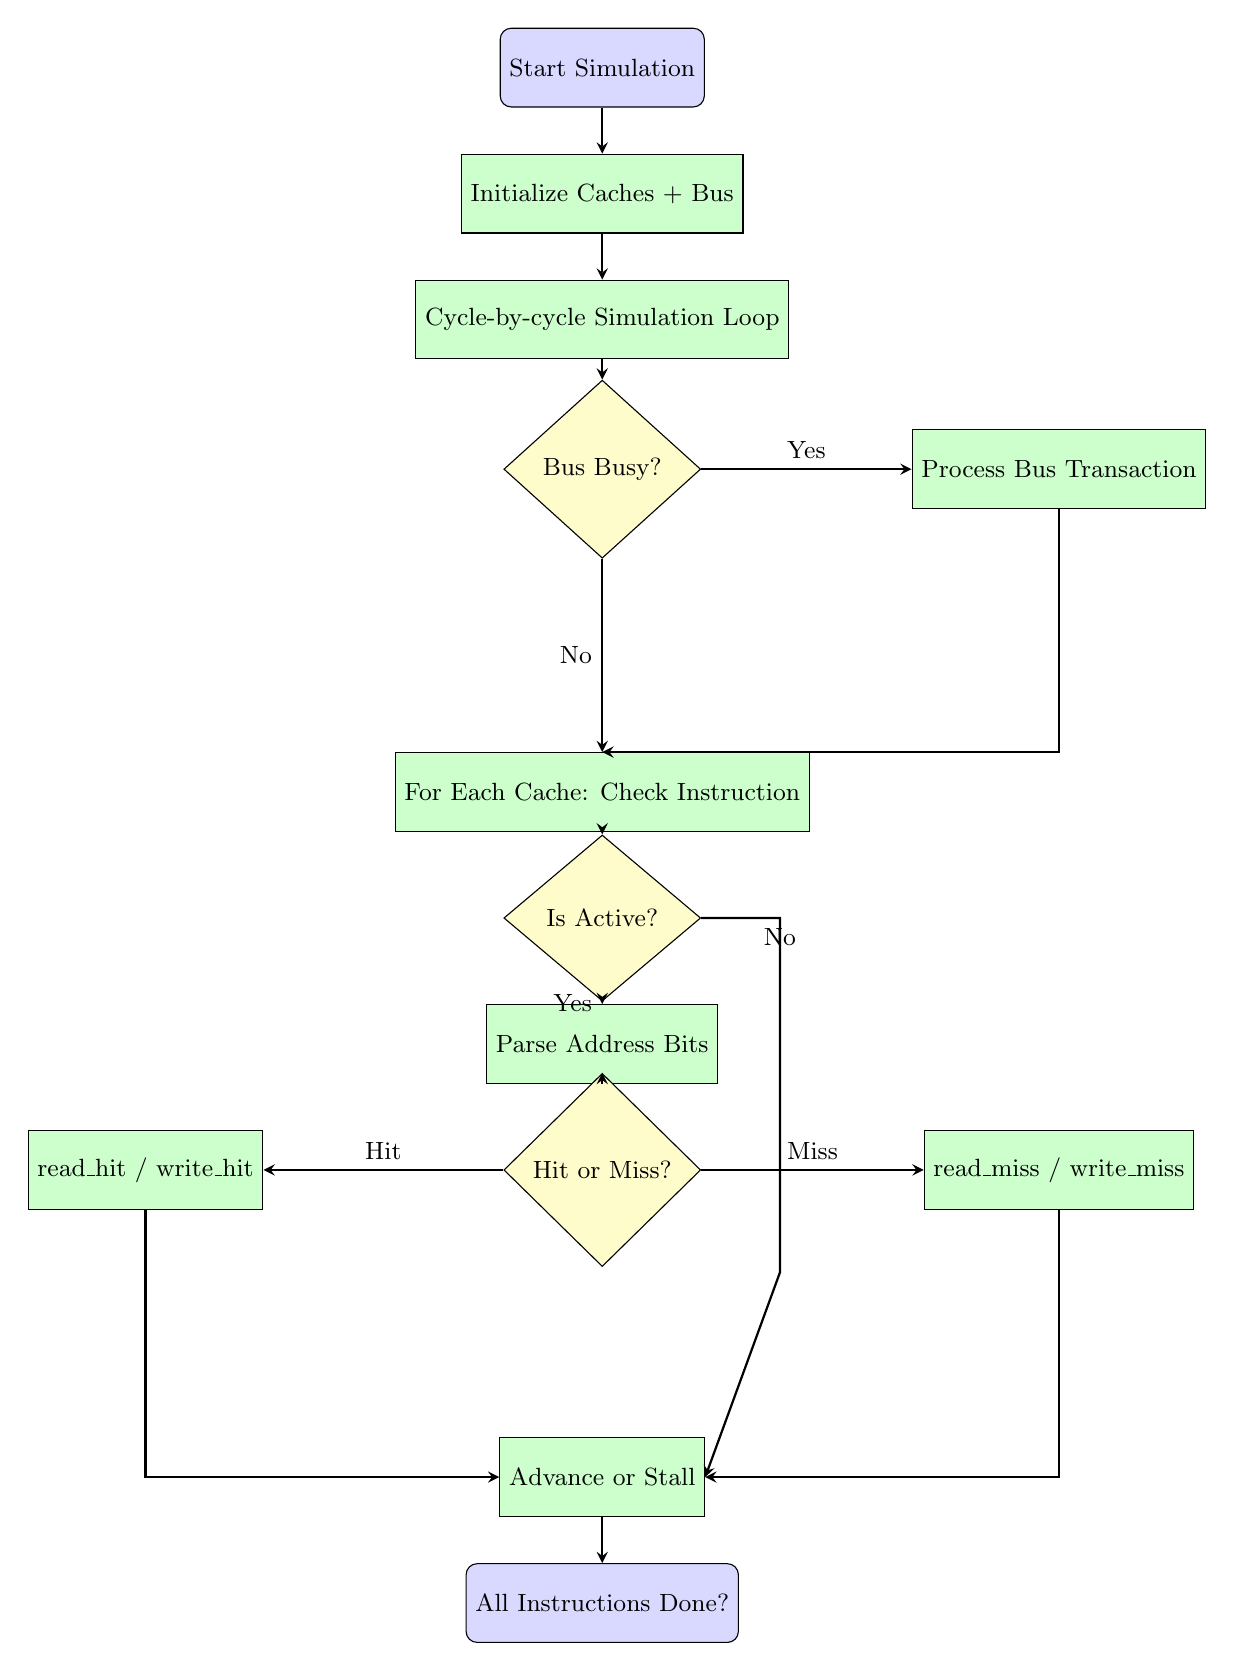
\begin{tikzpicture}[node distance=1.6cm, every node/.style={font=\small}]
\tikzstyle{startstop} = [rectangle, rounded corners, minimum width=2.5cm, minimum height=1cm,text centered, draw=black, fill=blue!15]
\tikzstyle{process} = [rectangle, minimum width=2.5cm, minimum height=1cm, text centered, draw=black, fill=green!20]
\tikzstyle{decision} = [diamond, minimum width=2.5cm, minimum height=1cm, text centered, draw=black, fill=yellow!20]
\tikzstyle{arrow} = [thick,->,>=stealth]

\node (start) [startstop] {Start Simulation};
\node (init) [process, below of=start] {Initialize Caches + Bus};
\node (loop) [process, below of=init] {Cycle-by-cycle Simulation Loop};
\node (buscheck) [decision, below of=loop, yshift=-0.3cm] {Bus Busy?};
\node (busproc) [process, right of=buscheck, xshift=4.2cm] {Process Bus Transaction};
\node (coreloop) [process, below of=buscheck, yshift=-2.5cm] {For Each Cache: Check Instruction};
\node (active) [decision, below of=coreloop] {Is Active?};
\node (parse) [process, below of=active] {Parse Address Bits};
\node (hitmiss) [decision, below of=parse] {Hit or Miss?};
\node (hit) [process, left of=hitmiss, xshift=-4.2cm] {read\_hit / write\_hit};
\node (miss) [process, right of=hitmiss, xshift=4.2cm] {read\_miss / write\_miss};
\node (wait) [process, below of=hitmiss, yshift=-2.3cm] {Advance or Stall};
\node (done) [startstop, below of=wait] {All Instructions Done?};

\draw [arrow] (start) -- (init);
\draw [arrow] (init) -- (loop);
\draw [arrow] (loop) -- (buscheck);
\draw [arrow] (buscheck) -- node[above]{Yes} (busproc);
\draw [arrow] (buscheck) -- node[left]{No} (coreloop);
\draw [arrow] (busproc.south) |- (coreloop.north);
\draw [arrow] (coreloop) -- (active);
\draw [arrow] (active) -- node[left]{Yes} (parse);
\draw [arrow] (parse) -- (hitmiss);
\draw [arrow] (hitmiss) -- node[above]{Hit} (hit);
\draw [arrow] (hitmiss) -- node[above]{Miss} (miss);
\draw [arrow] (hit.south) |- (wait.west);
\draw [arrow] (miss.south) |- (wait.east);
\draw [arrow] (wait) -- (done);
\draw [arrow] (active.east) -- ++(1,0) node[below]{No} -- ++(0,-4.5) -- (wait.east);
\end{tikzpicture}
\vspace{0.3cm}

\textbf{Figure:} Simulation control flow between bus and cache processors
\end{center}
\subsection{False Sharing}
We have shown the false sharing by comparing two different apps doing identical operations but one causes false sharing while other does not.
\begin{figure}[H]
        \centering
        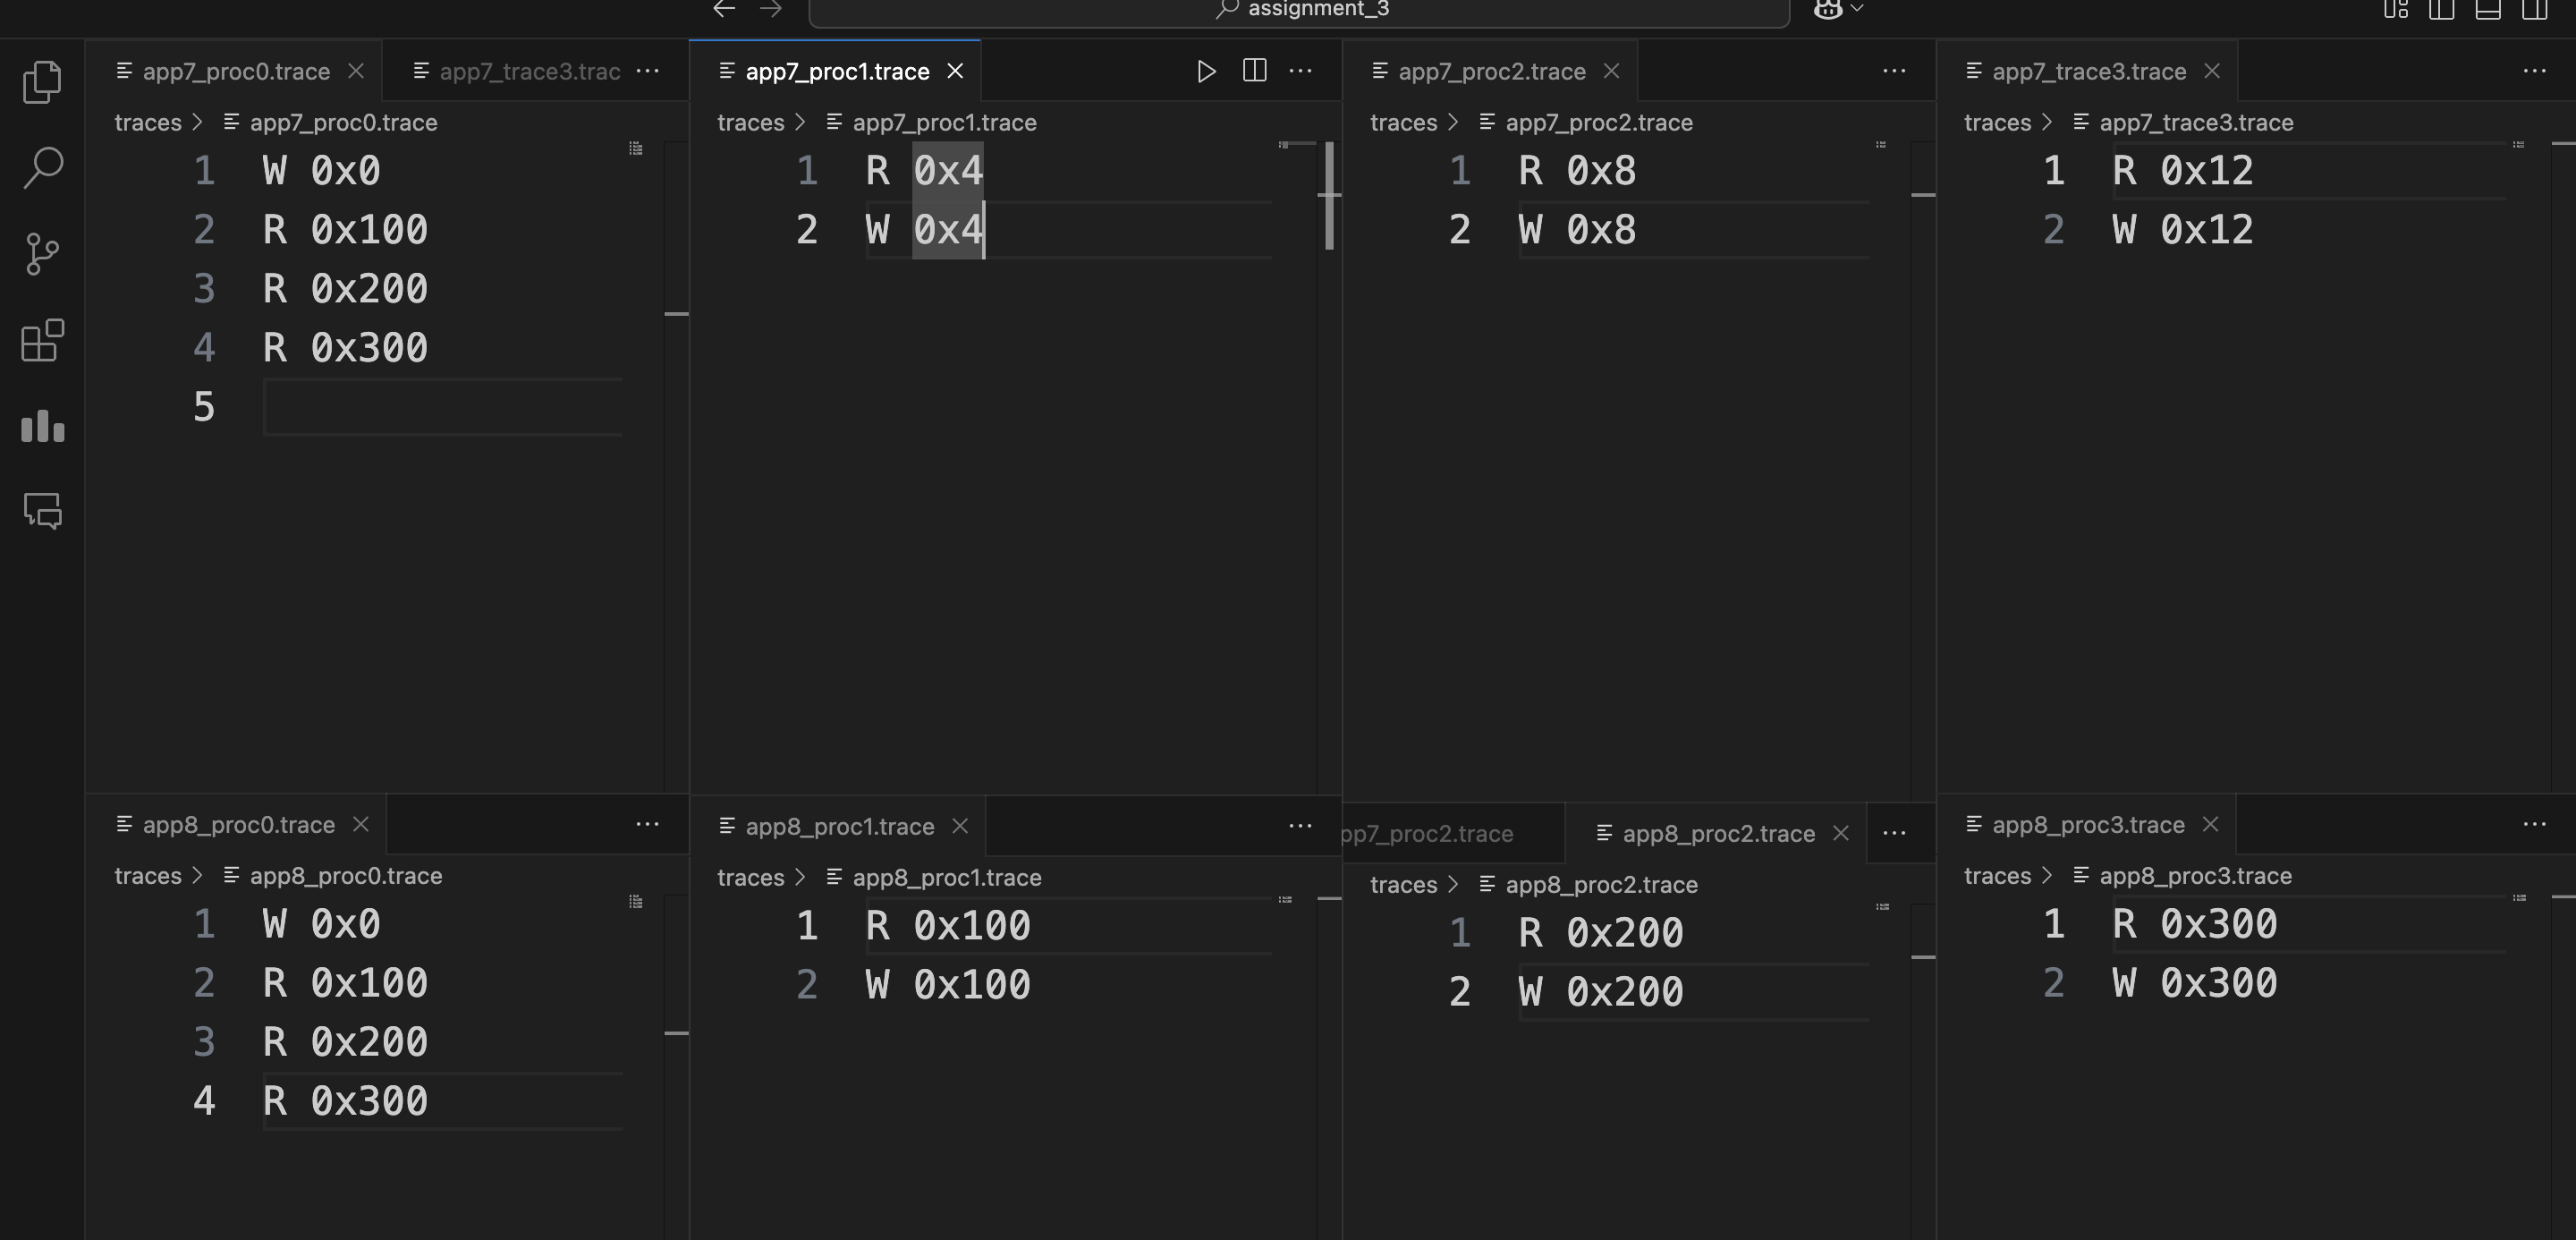
\includegraphics[width=0.7\textwidth]{false.png}
        \caption{False Sharing Traces}
        \label{fig:fixed_size_variation}
    \end{figure}
In both the apps in trace0 we have did 4 reads which all will get miss consuming the accounting for 400 cycles in both the apps.

Then from trace1 onwards each trace does a read and then a write on some address, in app1 all the addressees are from the same cache line so each one will be a cache miss and data will come from the cache0 via bus , in app2 all the adress belong to different cachelines in core 0 so here also the data come from cache 0 via bus.

Then there is a local write hit in each process so one would expect similar number of cycles in both the apps, but the here comes the false sharing in app1 all the adressess are from the same cache line so when one core has a read miss then it has to take data from the previous core but  the previous core has the same cache line in modified state which has to be written back into memory causing 100 cycles delay, this happen for all the three cores leading to a differnce of 300 cycles as can bee seen in the output.

 \begin{figure}[H]
        \centering
        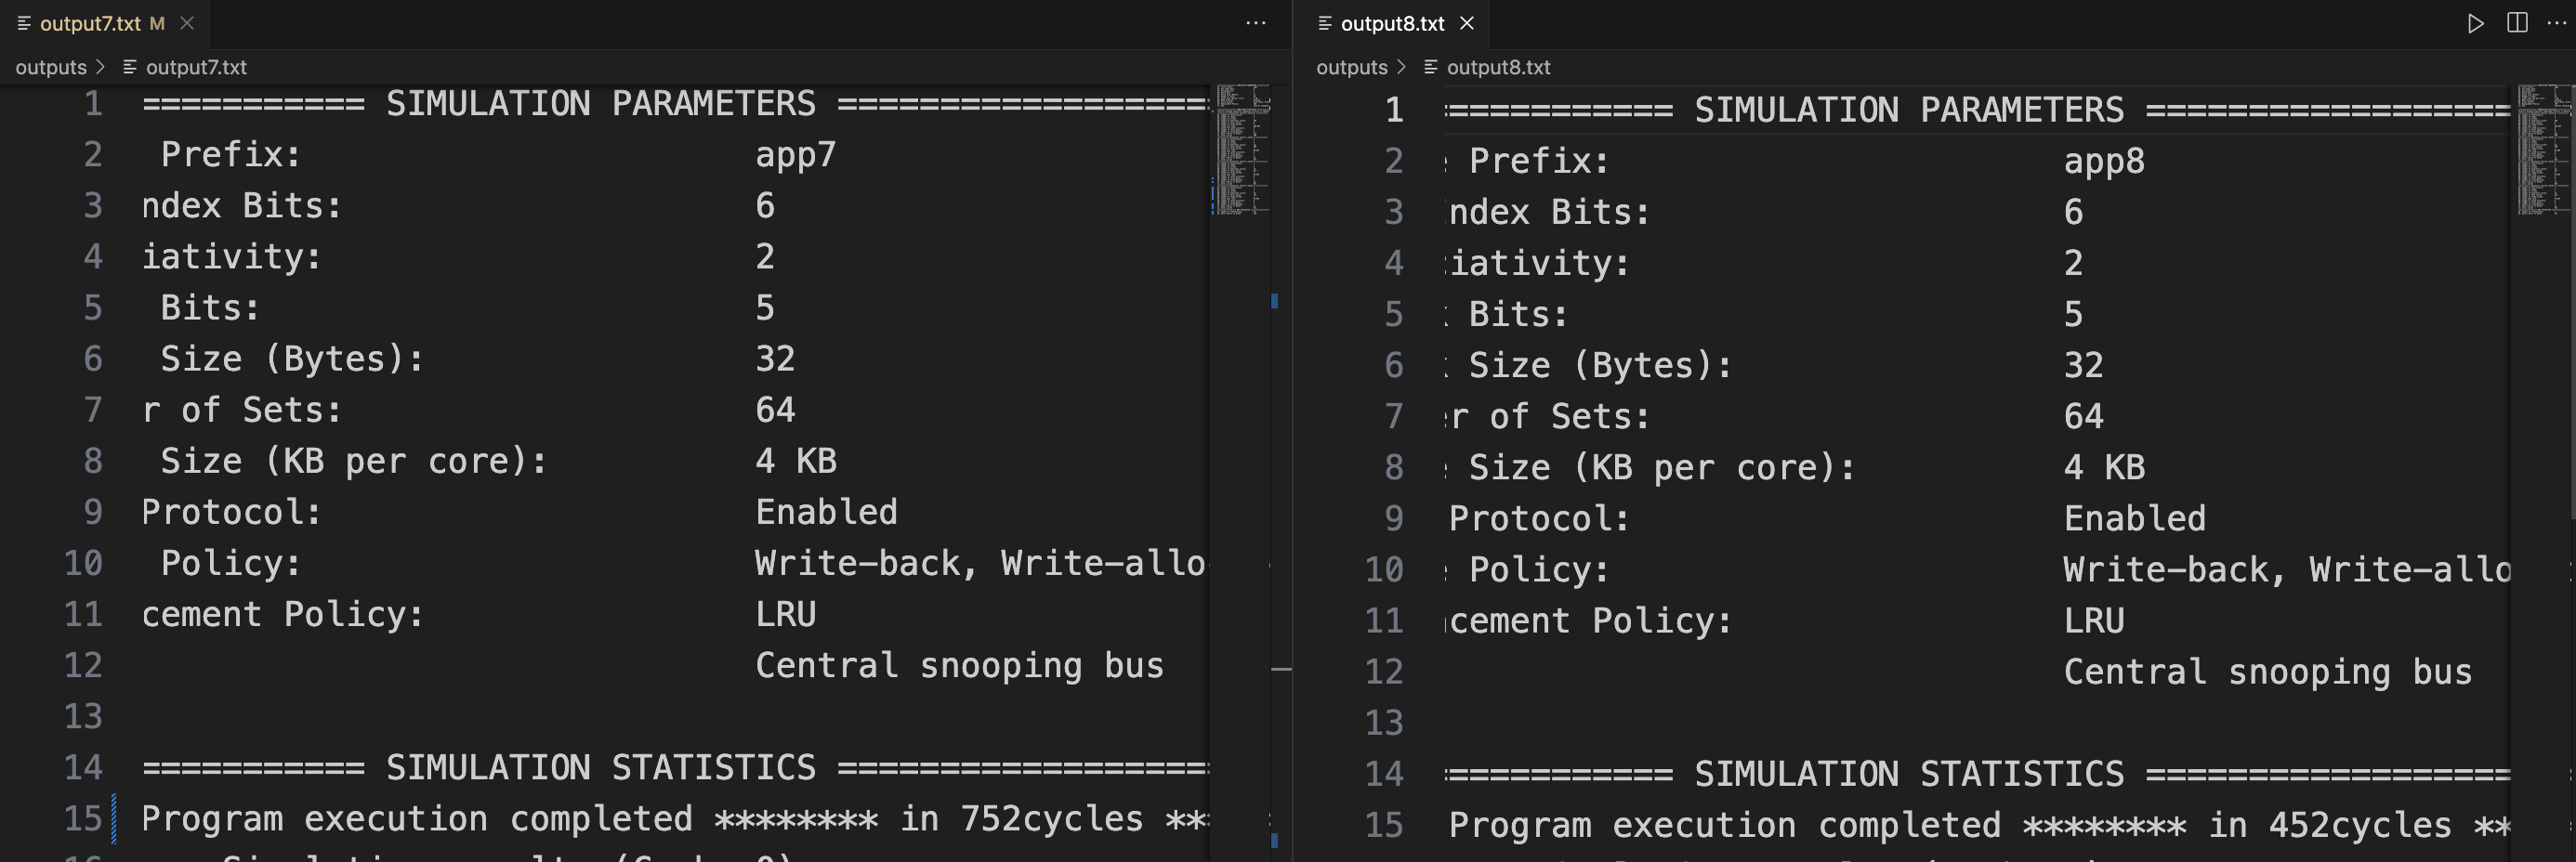
\includegraphics[width=0.7\textwidth]{false_output.png}
        \caption{False Sharing Output}
        \label{fig:fixed_size_variation}
    \end{figure}

\subsection{Test Traces Analysis}

\begin{itemize}
    \item \textbf{App3:} In this trace, every core writes to the same memory location. On a write miss, a core may find the block in another cache in the \texttt{M} (Modified) state. The owning cache must first write the data back to memory before the requesting cache can fetch it. This results in additional delays, leading to approximately \textbf{300 extra cycles} compared to \textbf{App5}, as shown in \texttt{output9.txt}.

    \item \textbf{App4:} This trace runs on a cache configuration with only one set. Initially, Core 0 reads from memory, followed by Core 1 writing to a different address. Then, Core 1 writes again to \texttt{0x0}, which was previously loaded by Core 0. This causes a write miss and triggers a bus transaction. Core 1 invalidates Core 0's block and prepares to write. However, due to the single-set constraint and presence of a block in \texttt{M} state, Core 1 must first write back the existing block before writing its own data. This showcases both invalidation and forced write-back due to limited associativity.

    \item \textbf{App5:} In this trace, each core reads from a different block. As a result, each core requires bus access during its execution phase. Since the bus is shared, this creates a \textbf{sequential execution} scenario. The total number of cycles required is \textbf{401}, as shown in \texttt{output5.txt}.

    \item \textbf{App6:} This test focuses on a single core performing reads from different addresses. Each read results in a miss and fetches data from memory. Other cores remain idle throughout, with \textbf{zero idle and execution cycles}. This demonstrates isolated execution. Refer to \texttt{output6.txt} for results.

    \item \textbf{App7 and App8:} These are analyzed under the \textbf{False Sharing} subsection of the report. App7 suffers from false sharing due to writes to addresses within the same cache line, causing unnecessary invalidations and write-backs, while App8 avoids this by writing to different cache lines.

    \item \textbf{App9:} This trace features reads to the \textbf{same memory location} from all cores. Since the data is already present in one core’s cache, \textbf{cache-to-cache transfers} occur, reducing memory access time. As a result, the execution time drops significantly to \textbf{149 cycles} (compared to 401 in App5). See \texttt{output9.txt}.

    \item \textbf{App10:} All cores perform writes to the same memory location. On a write miss, if another cache holds the block in \texttt{M} state, it must first write it back. Then the requesting cache fetches the data from memory. This results in \textbf{300 additional cycles} compared to App5, as shown in \texttt{output10.txt}.
\end{itemize}




\end{document}
